
\newcommand{\nomedoc}{Manuale Utente}
\newcommand{\versione}{1.0}
\newcommand{\versioneglossario}{3.0}
\newcommand{\versionenormeprogetto}{3.0}
\newcommand{\nomefile}{ManualeUtente-\versione.pdf}
\newcommand{\datacreazione}{24 Febbraio 2011}
\newcommand{\datamodifica}{27 Febbraio 2011}
\newcommand{\stato}{formale}
\newcommand{\uso}{esterno}
\newcommand{\redazione}{Baron Federico}
\newcommand{\verifica}{Cosimo Caputo}
\newcommand{\approvazione}{Mandolo Andrea}
\newcommand{\distribuzione}{
VT.G \\
& Prof. Vardanega Tullio\\
& Prof. Cardin Riccardo }

% FUNZIONI TIPOGRAFICHE
\newcommand{\co}{\texttt} % courier
\newcommand{\bo}{\textbf} % bold
\newcommand{\pr}{\par\medskip} % paragrafo spaziato
\newcommand{\sca}{\textsc} % small caps

\documentclass[a4paper,12pt]{report}
% 10pt,11pt,12pt
% titlepage, notitlepage -> per dare inizio o no ad una nuova pagina dopo titolo
% twoside -> per dire se fronte-retro
\usepackage[latin1]{inputenc}
% per caratteri accentati
\usepackage[italian]{babel}
% per regole sintattiche italiane
\usepackage[bookmarks=true, pdfborder={0 0 0 0}]{hyperref}
% per collegamenti ipertestuali
\usepackage{graphicx}
% per inserimento immagini

% \usepackage{enumerate}
% per personalizzare elenchi puntati

\usepackage[hmargin=2cm]{geometry} %margine 2 cm
%\geometry{options varie}

% comandi per gestire meglio header e footer
\usepackage{fancyhdr}  % header e footer
\usepackage{totpages}
\pagestyle{fancy}
\renewcommand{\headrulewidth}{0.4pt}
\renewcommand{\footrulewidth}{0.4pt}

\setlength{\headheight}{1.2cm} % NON TOCCARE
\setlength{\voffset}{-1.5cm} % NON TOCCARE
\setlength{\textheight}{666pt} % NON TOCCARE
\setlength{\footskip}{60pt}
\setlength{\parindent}{0pt} % INDENTAZIONE

\lhead{\nomedoc\  (ver. \versione)}
\chead{}
\rhead{
\includegraphics[height=1cm]{img/netmus.png}}
\lfoot{
\includegraphics[height=0.8cm]{img/logo.png}}
\cfoot{}
\rfoot{\thepage}

\usepackage{titlesec}
\titleformat{\chapter}{\normalfont\huge\bfseries}
{\thechapter}{20pt}{\Huge}

\usepackage{rotating}   % PER TABELLE E AMBIENTI RUOTATI
\usepackage{array}
\usepackage{color}
\usepackage{colortbl}  % VARIE PER GESTIRE I COLORI
\definecolor{Orange}{RGB}{255,127,0}   % ARANCIO ACCES0
\definecolor{orange}{RGB}{255,207,80}  % ARANCIO TENUE

\addtocontents{toc}{\protect\thispagestyle{fancy}}  % PER INDICI CON + PAGINE
\usepackage[font=it]{caption}    % PER RENDERE CORSIVE LE DIDASCALIE
\usepackage{eurosym}  % PER SIMBOLO EURO

% \usepackage{listings}   per codice sorgente

\author{VT.G - Valter Texas Group}

\begin{document}

\pagenumbering{Roman} % INIZIO NUMERAZIONE ARABA

\vspace*{1cm}
\begin{center}

\begin{LARGE} \sca{Federico Baron} \end{LARGE}\\
\vspace{0.5cm}
\begin{Large}
\emph{fede.baron.89@gmail.com} \end{Large}\\
\vspace*{1cm} 
\includegraphics[width=5cm]{img/logo.png}\\
\vspace{0.5cm}
\begin{Large} \emph{``Comunicazione Aumentata/Alternativa per Giovani Ospiti
della Terapia Intensiva Pediatrica''} \end{Large}\\
\vspace{3cm}
\begin{Large} \sca{\nomedoc} \end{Large}\\
\end{center}
\vspace{1cm}

% INFORMAZIONI DOCUMENTO
\begin{center}
\begin{tabular}{r|l}
\hline & \\
\bo{Nome} & \nomefile \\
\bo{Versione attuale} & \versione \\
\bo{Data creazione} & \datacreazione \\
\bo{Data ultima modifica} & \datamodifica \\
\bo{Redazione} & \redazione \\
& \\\hline
\end{tabular}
\end{center}
\newpage

\chapter*{Sommario}
\thispagestyle{fancy}
Il presente documento fornisce una guida chiara e semplice per l'utilizzo del
sistema NetMus.\\
Comprende un glossario con i termini meno conosciuti e un'appendice con i
problemi pi\` comuni, possibili cause e soluzioni proposte.

\newpage
% REGISTRO MODIFICHE
\section*{Registro delle modifiche}

\begin{longtable}{|p{0.13\textwidth}|c|p{0.2\textwidth}|p{0.46\textwidth}|}
\hline
\rowcolor{orange} \bo{Data} & \bo{Versione} & \bo{Autore} & \bo{Descrizione} \\
\hline
\endhead
\hline
\endfoot
28/02/2011 & 1.0 & Mandolo Andrea & Validazione per consegna RQ.\\
\hline
28/02/2011 & 0.9 & Cosimo Caputo & Verificato l'intero documento.\\
\hline
27/02/2011 & 0.8 & Baron Federico & Corretti errori e Sistemata impaginazione
immagini.\\
\hline 
27/02/2011 & 0.7 & Palazzin Alberto & Aggiornato glossario, corretti un p\`o di
errori.\\
\hline
27/02/2011 & 0.6 & Daminato Simone & Inseriti gli screenshot nel documento.\\
\hline
26/02/2011 & 0.5 & Caputo Cosimo & Inizio creazione glossario.\\
\hline
26/02/2011 & 0.4 & Palazzin Alberto & Aggiunte nuove azioni possibili nella sezione
"Istruzioni per l'uso".\\
\hline
25/02/2011 & 0.3 & Baron Federico & Stesa parte preliminare delle istruzioni per
l'uso.\\
\hline
24/02/2011 & 0.2 & Daminato Simone & Stesura preambolo.\\
\hline 
24/02/2011 & 0.1 & Mandolo Andrea & Stesura prima versione del Manuale Utente.\\

\end{longtable}

% INDICE
\tableofcontents

\chapter{Introduzione}
\thispagestyle{fancy} % serve perche' nelle pagine di inizio Chapter esca header e footer
\pagenumbering{arabic} % INIZIO NUMERAZIONE NORMALE
\rfoot{\thepage\ di \pageref{TotPages}}
Questo manuale \`e destinato agli utilizzatori di \co{NetMus}, e comprende una
descrizione del prodotto e le istruzioni per l'uso, oltre a due appendici
riportanti gli eventuali messaggi di errore e il glossario.\\

Tutti i termini presenti nel glossario a termine del documento sono sottolineati
alla prima occorrenza \underline{in questo modo}.

\section{Definizione dell'utente del prodotto}
\co{NetMus} pu\`o essere utilizzato da chiunque: sono richieste solo poche
nozioni di base, ovvero come navigare in internet utilizzando un
\underline{browser web}.

\section{Come leggere il manuale}
Questo manuale presenta il prodotto \co{NetMus} e descrive le sue funzionalit\`a
e l'approccio dell'utente al suo utilizzo. In particolare, verranno illustrate
le azioni che l'utente pu\`o effettuare con questo software e come risolvere, se
possibile, gli eventuali problemi riscontrabili durante il suo l'utilizzo.

\section{Documenti utili}
I documenti a cui ci si  riferiti per stendere il presente documento, e che
possono tornare utili per la lettura dello stesso, sono:
\begin{itemize}
  \item Analisi dei requisiti v3.0
  \item Norme di progetto v3.0
  \item Piano di progetto v3.0
  \item Specifica tecnica v2.0
  \item Definizione del prodotto v1.0
  \item Piano di qualifica v3.0
  \item Verbale 1 v1.0
  \item Capitolato C2 - NetMus del corso di Ingegneria del Software, A.A.
2010/11 (disponibile all'indirizzo web
\url{http://www.math.unipd.it/~tullio/IS-1/2010/Progetto/NetMus.pdf})
\end{itemize}

\section{Come riportare problemi e malfunzionamenti}
Per segnalare problemi e malfunzionamenti \`e disponibile un servizio online a
questo indirizzo: \url{http://code.google.com/p/netmus/issues/list}.\\
\`E sufficiente cliccare in alto a sinistra su \emph{New issue}, e nel modulo
compilare i campi col titolo e la descrizione del problema.
Come aiuto per descrivere il problema, consigliamo di selezionare il template
\emph{Defect report from user}, che contiene una traccia che aiuta ad inserire
tutte le informazioni necessarie.

\chapter{Descrizione generale}
\thispagestyle{fancy}
Oggigiorno, la maggior parte della musica che ascoltiamo \`e in formato digitale: \`e
per questo che nasce \co{NetMus}, uno strumento per gestire e condividere le
nostre canzoni preferite, che sfrutta le nuove tecnologie, come il
\underline{cloud computing}.\\

\co{NetMus} permette agli utenti di avere una
libreria virtuale online con tutte le canzoni che si ascoltano abitualmente, in modo da
poterle ascoltare ovunque ci si trovi, e condividerle con altri utenti.\\

Oltre alla comodit\`a di poter accedere alla propria libreria musicale, il
sistema \co{NetMus} svolge il ruolo anche da semplice ``\underline{social
network}'' che permette di interagire con gli altri utenti iscritti. \`E quindi
possibile visualizzare e riprodurre i cataloghi multimediali degli altri utenti, oltre che
creare una lista di amici con qualunque utente si voglia.\\

Il prodotto \`e molto facile da utilizzare, una volta effettuato l'accesso
a \co{NetMus} basta collegare il proprio lettore mp3 e lasciarlo lavorare in
automatico, oppure indicargli in che cartella si tengono le canzoni: tutte le 
informazioni verranno estratte, analizzate, completate e
inserite nel nostro profilo, pronte per essere utilizzate.\\

Tra le possibilit\`a offerte, troviamo sia lo \underline{streaming} audio che
quello video, il completamento automatico delle informazioni dei brani, le playlist, e
molto altro.\\

Il tutto \`e implementato con un'interfaccia grafica molto semplice che fornisce
tutte le funzionalit\`a necessarie, ma nonostante la sua semplicit\`a ha
un'impatto visivo notevole.
\chapter{Istruzioni per l'uso}
\thispagestyle{fancy}

\section{Descrizione funzionale}

\subsection{Registrazione a NetMus}
Per iniziare ad utilizzare NetMus collegarsi all'indirizzo
\url{http://netmusbeta.appspot.com} . \\
\begin{figure}[htbp]
  \centering
  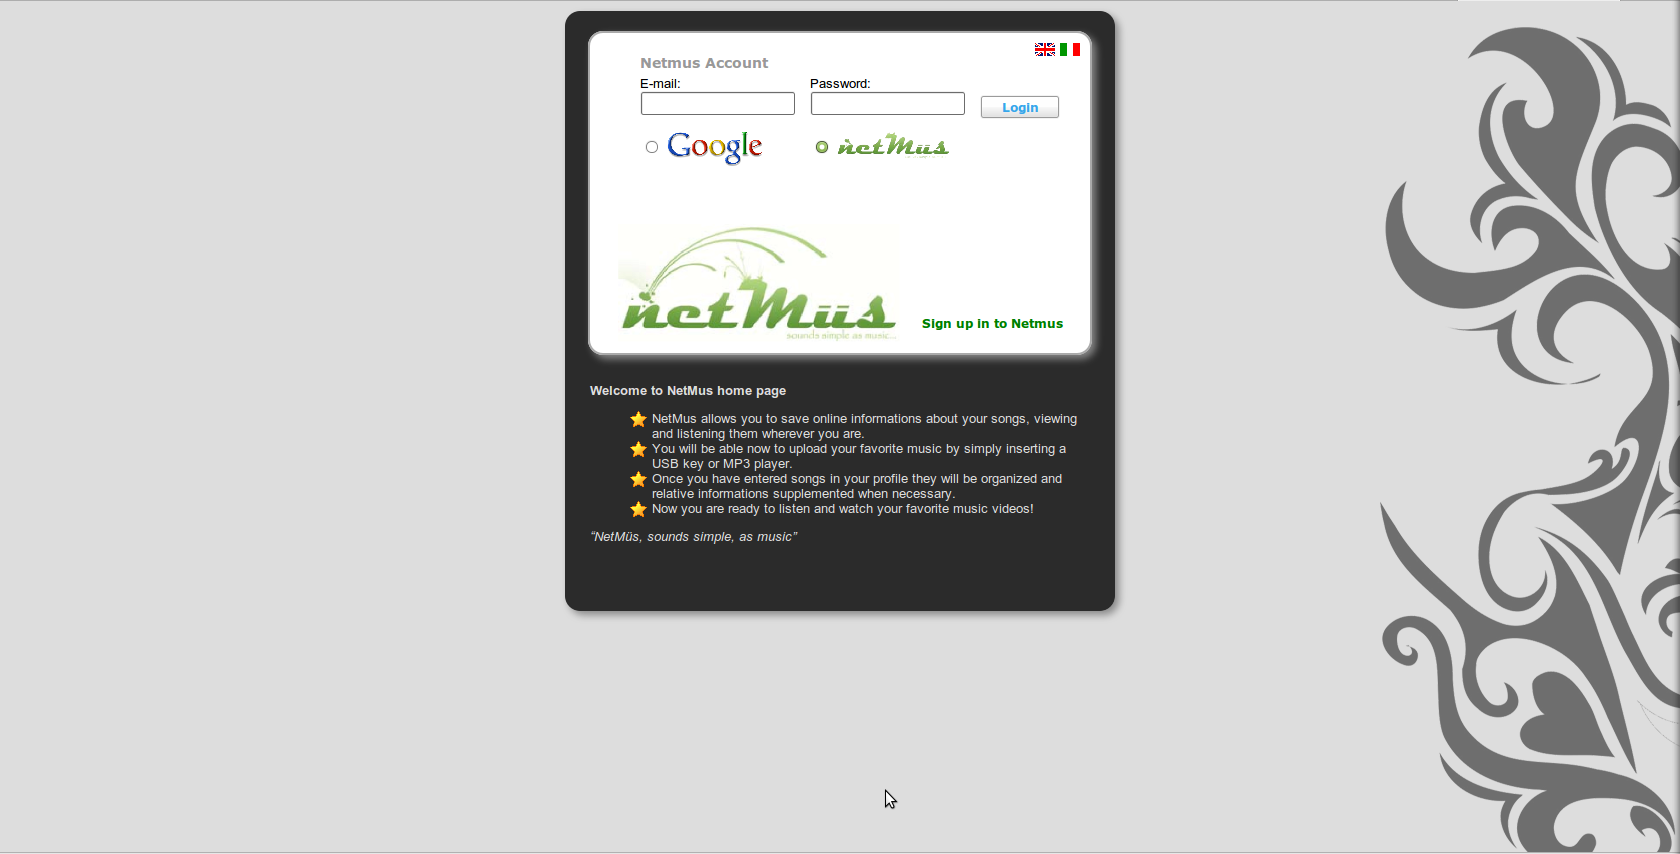
\includegraphics[width=15cm]{img/MU/login.png}
\caption{Interfaccia di NetMus Login}
\end{figure}
Qui vi verr\`a presentata la pagina di login per
accedere al sistema. Se possedete gi\`a un account Google, potete effettuare
l'accesso direttamente con i dati dell'account di Google, dato che il sistema
lo permette.\\
\begin{figure}[htbp]
  \centering
  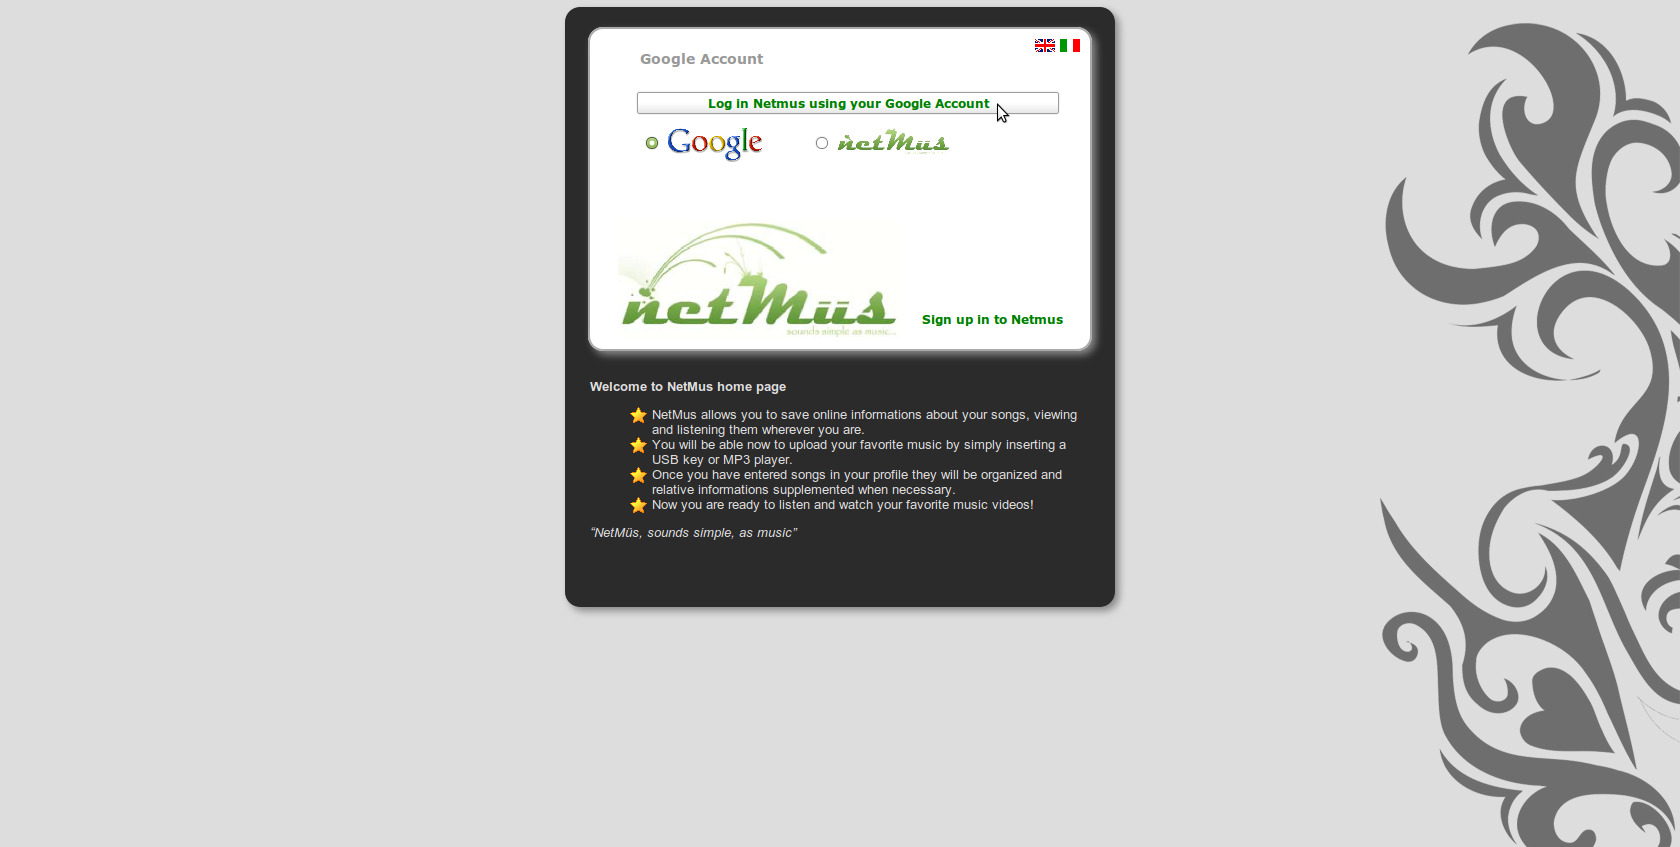
\includegraphics[width=15cm]{img/MU/loginGoogle.png}\\
\caption{Interfaccia per il Login Google}
\end{figure}

Se invece non siete utenti Google e questo
\`e il primo accesso, \`e necessario che vi registriate al sistema. La
registrazione cos\`i come l'utilizzo del sistema \co{NetMus} sono completamente
gratuiti.\\
\begin{figure}[htbp]
  \centering
  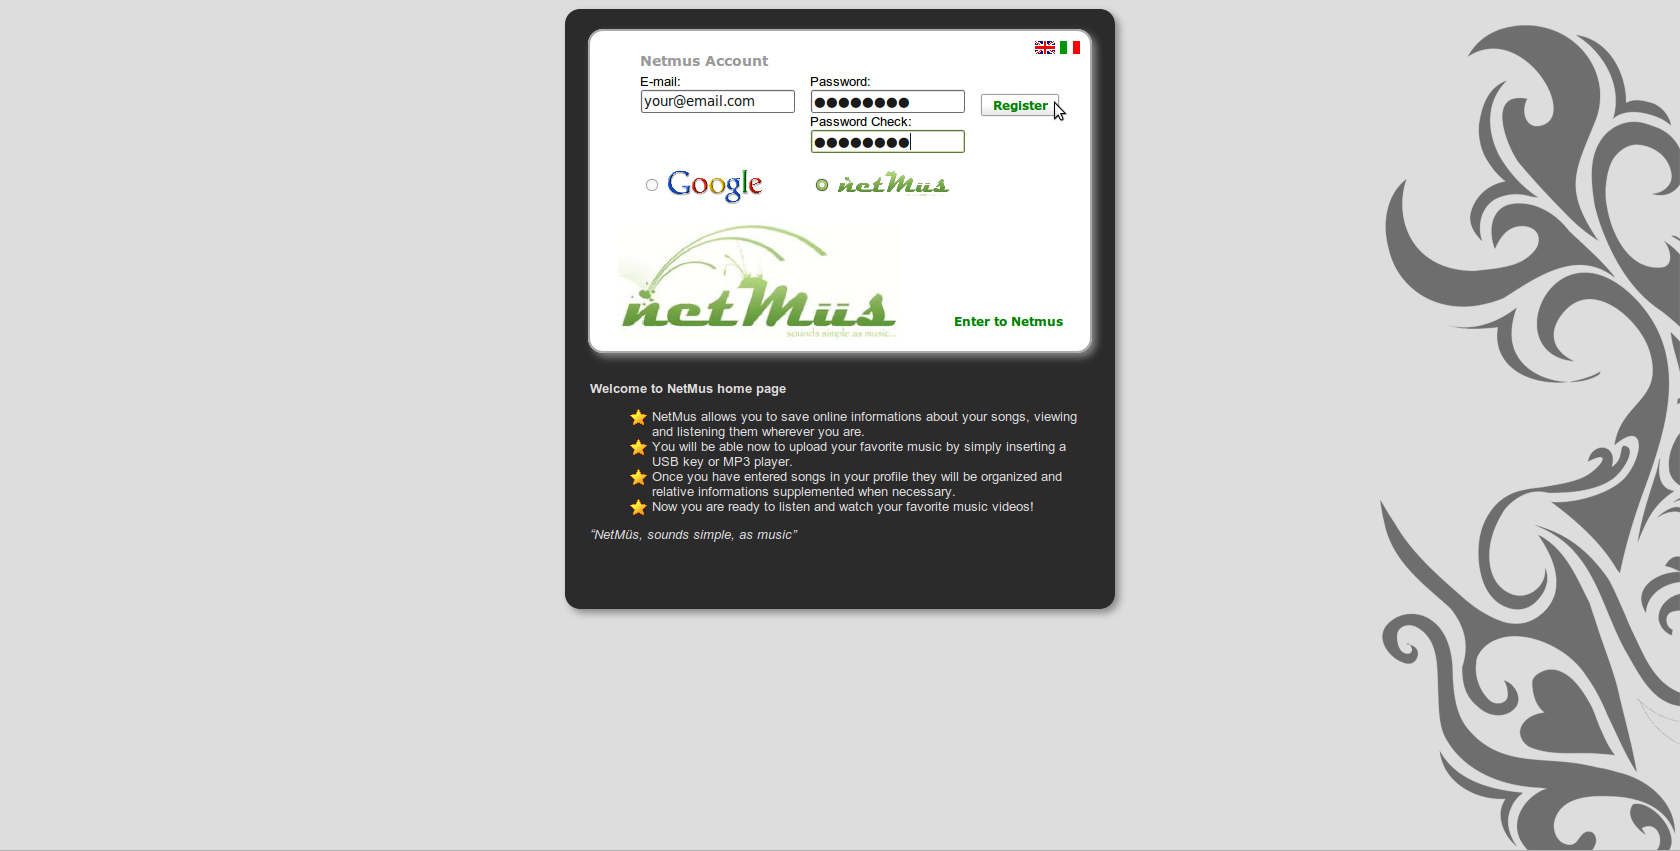
\includegraphics[width=15cm]{img/MU/registration.png}\\
\caption{Interfaccia di registrazione}
\end{figure}

La registrazione richiede un' email valida e una password di lunghezza maggiore
di 5 caratteri. Vi verr\`a inviata una mail all'indirizzo indicato che richiede
conferma per l'attivazione dell'account.\\
Una volta attivato il vostro account, avrete libero accesso al sistema
\co{NetMus}.

\subsection{Primo accesso a NetMus}

Al vostro primo accesso al sistema, l'interfaccia che vi verr\`a presentata
sar\`a strutturata in questo modo.\\
\begin{figure}[htbp]
  \centering
  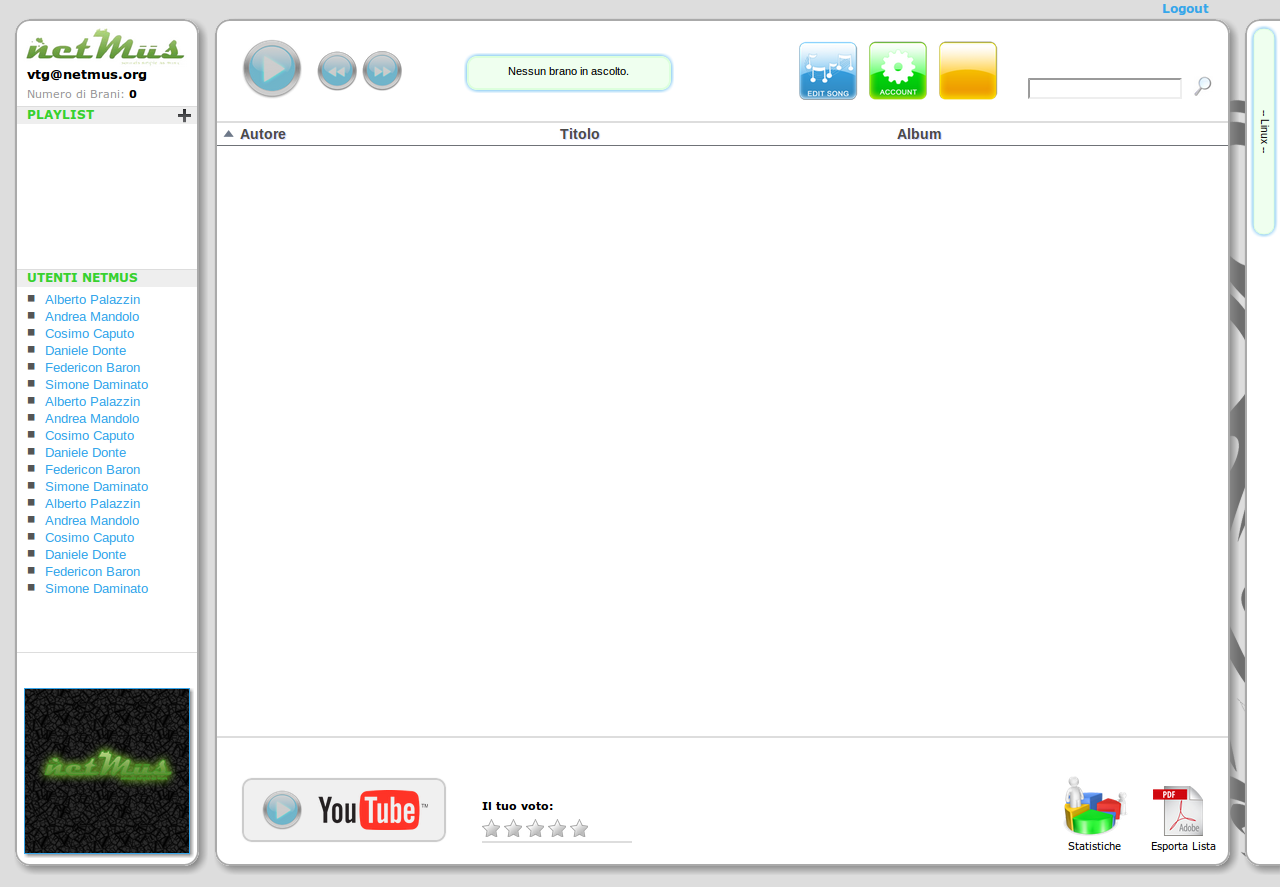
\includegraphics[width=15cm]{img/MU/profile_blank.png}\\
\caption{Pagina principale di NetMus al primo accesso}
\end{figure}

Un men\`u a sinistra presenta il logo del sistema, la mail con cui siete
registrati che viene utilizzato come vostro \underline{nickname}, e il numero di
brani presente nel vostro catalogo, che sar\`a pari a zero. Questo \`e il men\`u
delle playlist, infatti qui verranno visualizzate tutte le vostre playlist
create e permette di crearne di nuove cliccando il tasto ``+'' presente.\\
\\
La sezione centrale dell'interfaccia \`e la pi\`u importante, \`e infatti il
nostro catalogo multimediale con player annessi e tasti per svariate azioni.\\
\\
All'estrema sinistra della pagina \`e presente la barra per la scansione
dei \underline{dispositivi di archiviazione} \underline{di massa}, chiamata
pi\`u semplicemente ``DEVICE SCANNER BAR''. Tale barra \`e visibile nella sua
completezza solo al passaggio del mouse sopra di essa. La barra permette la
scansione manuale e visualizza l'avanzamento dell'analisi ed estrazione
automatica o manuale dei file mp3 da un dispositivo o da una \underline{directory}
selezionata.\\
\begin{figure}[htbp]
  \centering
  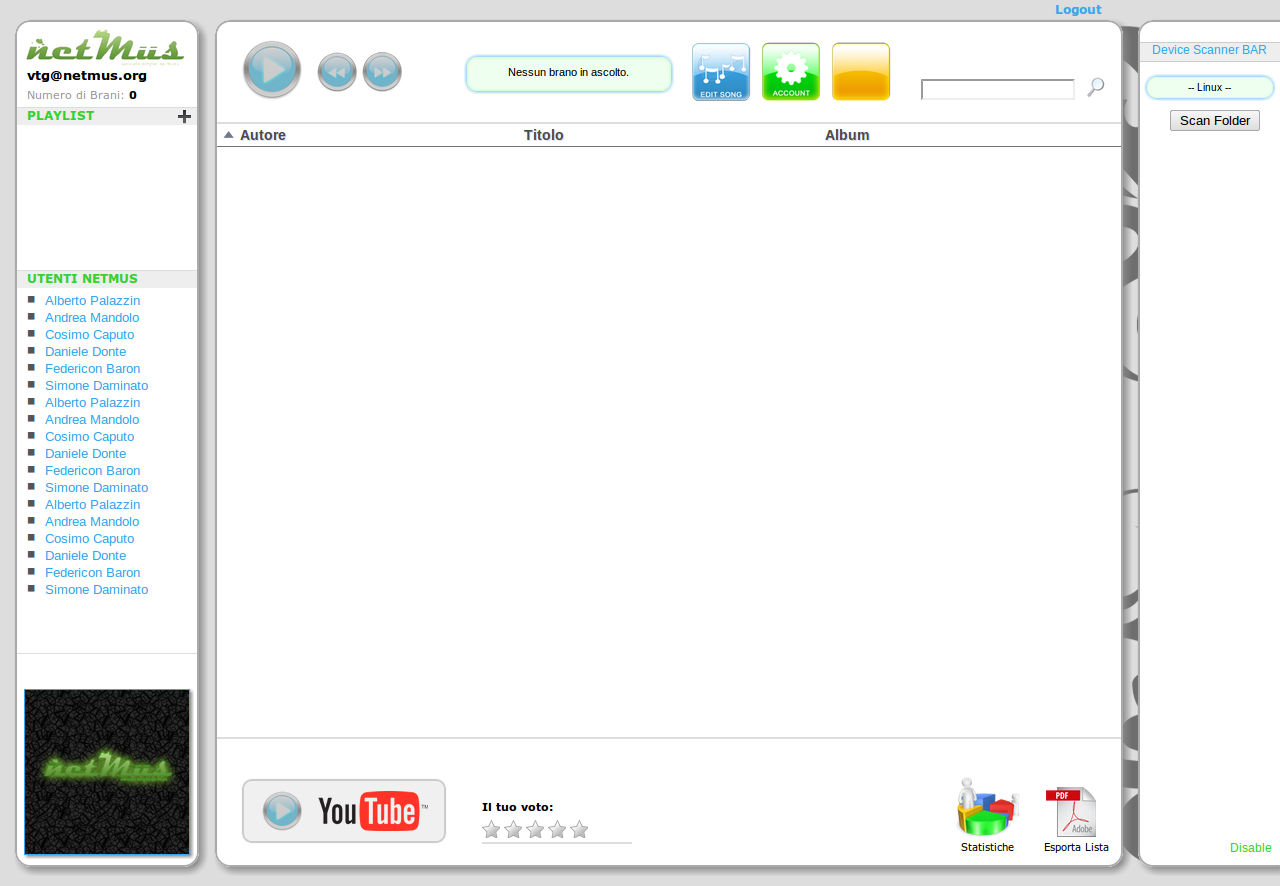
\includegraphics[width=15cm]{img/MU/applet_bar_open.png}\\
\caption{Pagina principale di NetMus con DEVICE SCANNER BAR espansa}
\end{figure} 


\newpage
\subsection{Iniziare ad utilizzare NetMus}

Per poter iniziare da subito a sfruttare la capacit\`a principale di \co{NetMus},
ossia quella di libreria musicale, \`e necessario inserire un dispositivo di
archiviazione di massa nella porta USB del proprio PC.\\
In alternativa \`e possibile scansionare qualunque directory del proprio PC
cliccando il tasto ``Scan Folder'' per la scansione manuale, e
selezionando la directory.\\
\begin{figure}[htbp]
  \centering
  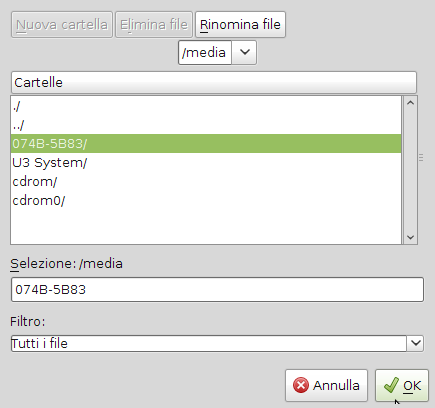
\includegraphics[width=15cm]{img/MU/scan_manual.png}\\ 
\caption{Interfaccia di selezione di una directory per la scansione
manuale}
\end{figure}

Quando parte l'analisi, nella DEVICE SCANNER BAR viene visualizzato
l'avanzamento del processo, che mostra il numero di file analizzati fino al
messaggio ``Sending Done'' che indica che i file sono stati inviati alla
libreria musicale.\\
\begin{figure}[htbp]
  \centering
  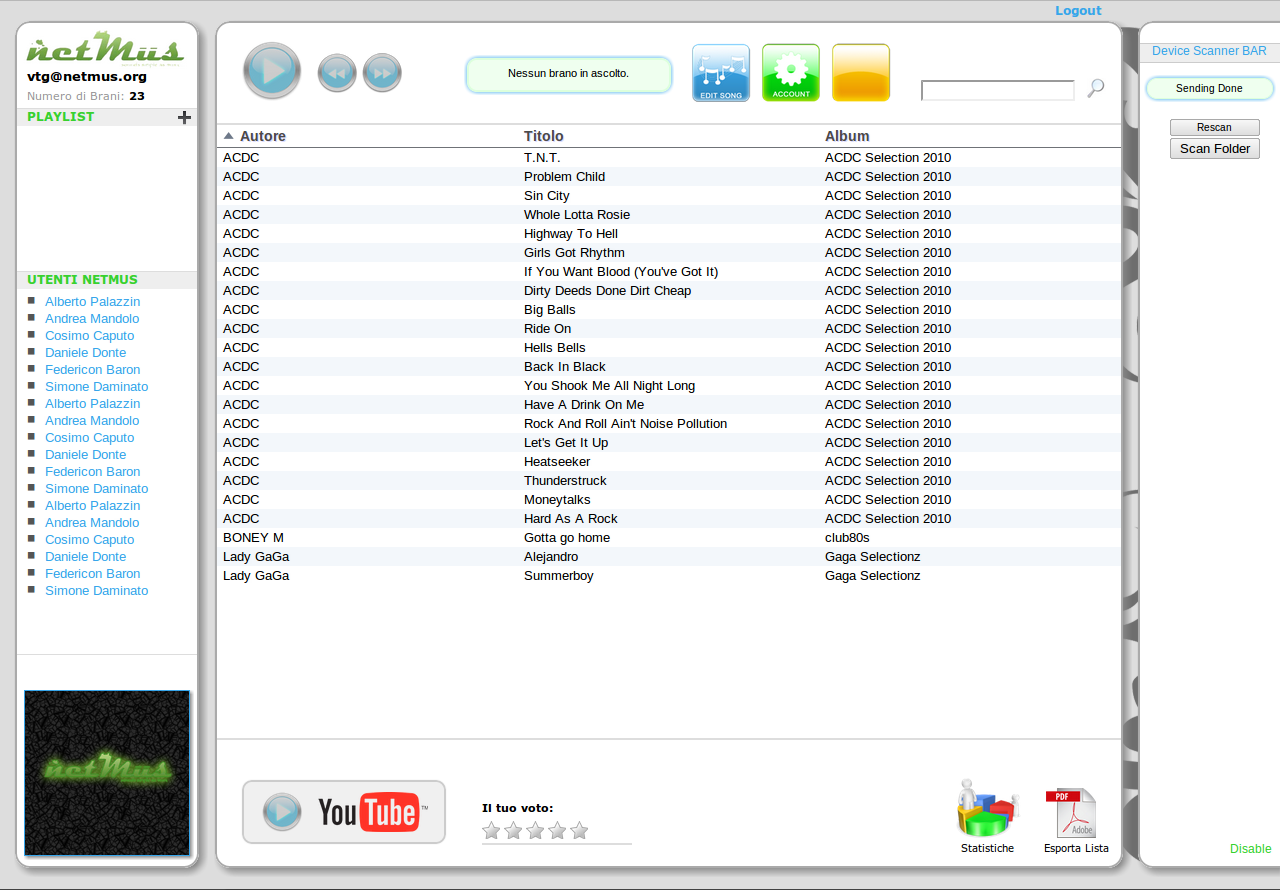
\includegraphics[width=15cm]{img/MU/song_loaded.png}\\
\caption{Interfaccia con catalogo multimediale caricato}
\end{figure}

Una volta inviati, i file dovrebbero comparire sul catalogo multimediale.\\
A questo punto \`e possibile iniziare a sbizzarrirsi con le funzionalit\`a di
\co{NetMus}. Le funzionalit\`a per comodit\`a di impostazione visiva e
sopratutto di ricerca, vengono elencate in sottoparagrafi.

\section{Azioni richieste/permesse}

\subparagraph{Ascoltare una canzone in streaming}

Come prima funzionalit\`a inseriamo la descrizione della pi\`u interessante
del nostro prodotto, ossia la riproduzione delle tracce in streaming.\\ Per
riprodurre una qualsiasi canzone del proprio catalogo, basta selezionarla nel
catalogo, quindi cliccare sul tasto play del \underline{player} in alto, o del
player YouTube in basso.\\
\begin{figure}[htbp]
  \centering
  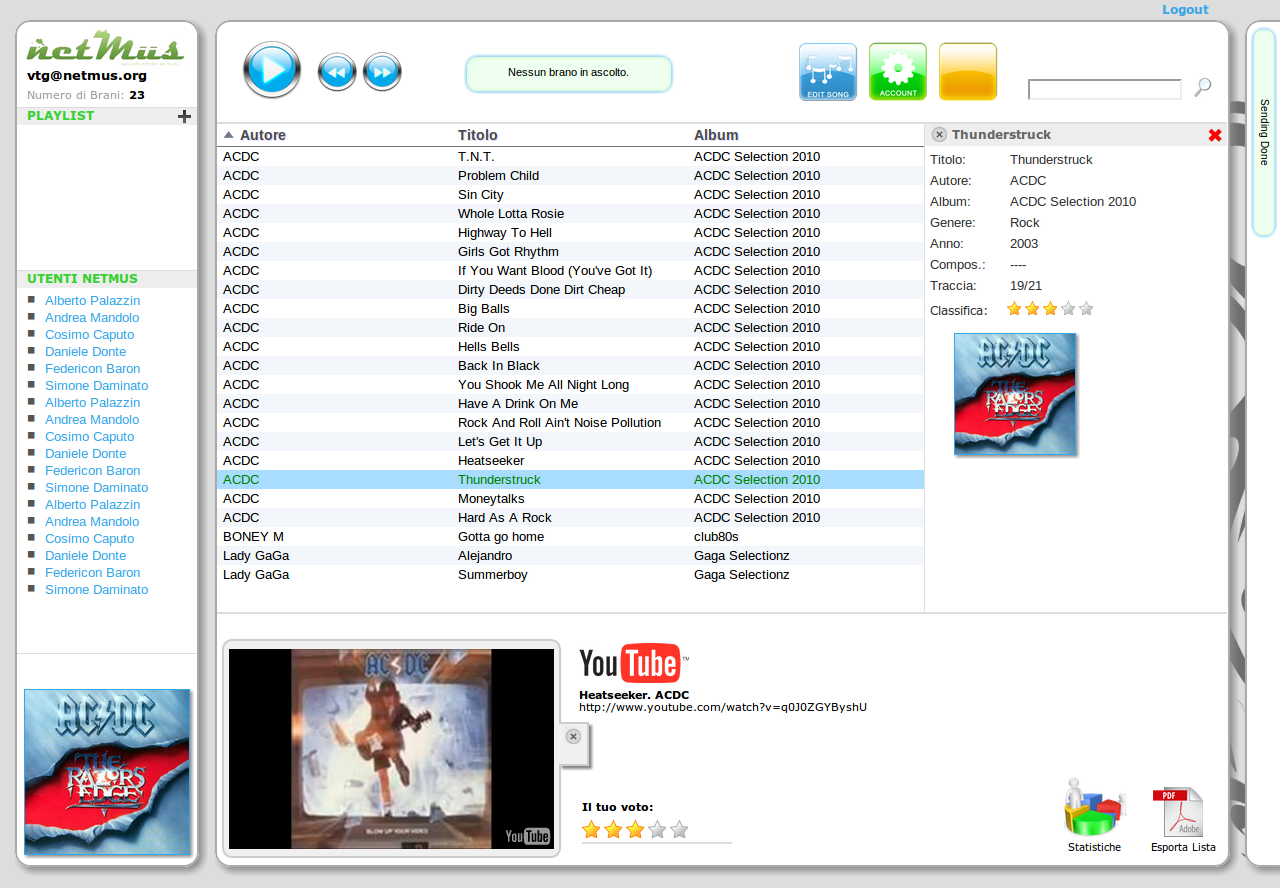
\includegraphics[width=15cm]{img/MU/player_youtube.png}\\
\caption{Interfaccia con riproduzione tramite player di YouTube}
\end{figure} 

Di fatto l'operazione svolta dai due player \`e la stessa, ma
si differenziano per il fatto che il player superiore permette riproduzione e
pausa dello stream audio, passaggio al brano precedente e successivo del catalogo, mentre il player
inferiore si trasforma in un riproduttore di video in streaming, in cui viene
riprodotto il video musicale della canzone trovato da YouTube.\\
Inoltre tale player evidenzia il link di YouTube a cui \`e stato trovato il
brano, e con un click il browser ci reindirizza a tale link.

\subparagraph{Creare Playlist}

La creazione di una \underline{playlist} \`e un'operazione molto semplice e
comoda per poter avere una sequenza delle canzoni preferite.\\
Per creare una playlist basta cliccare sul tasto ``+'' nel men\`u a sinistra di
fianco alla voce ``PLAYLIST''. Subito sotto comparir\`a un campo in cui
inserire il titolo della playlist. Una volta inserito il titolo e premuto invio,
la playlist sar\`a stata creata.\\
\begin{figure}[htbp]
  \centering
  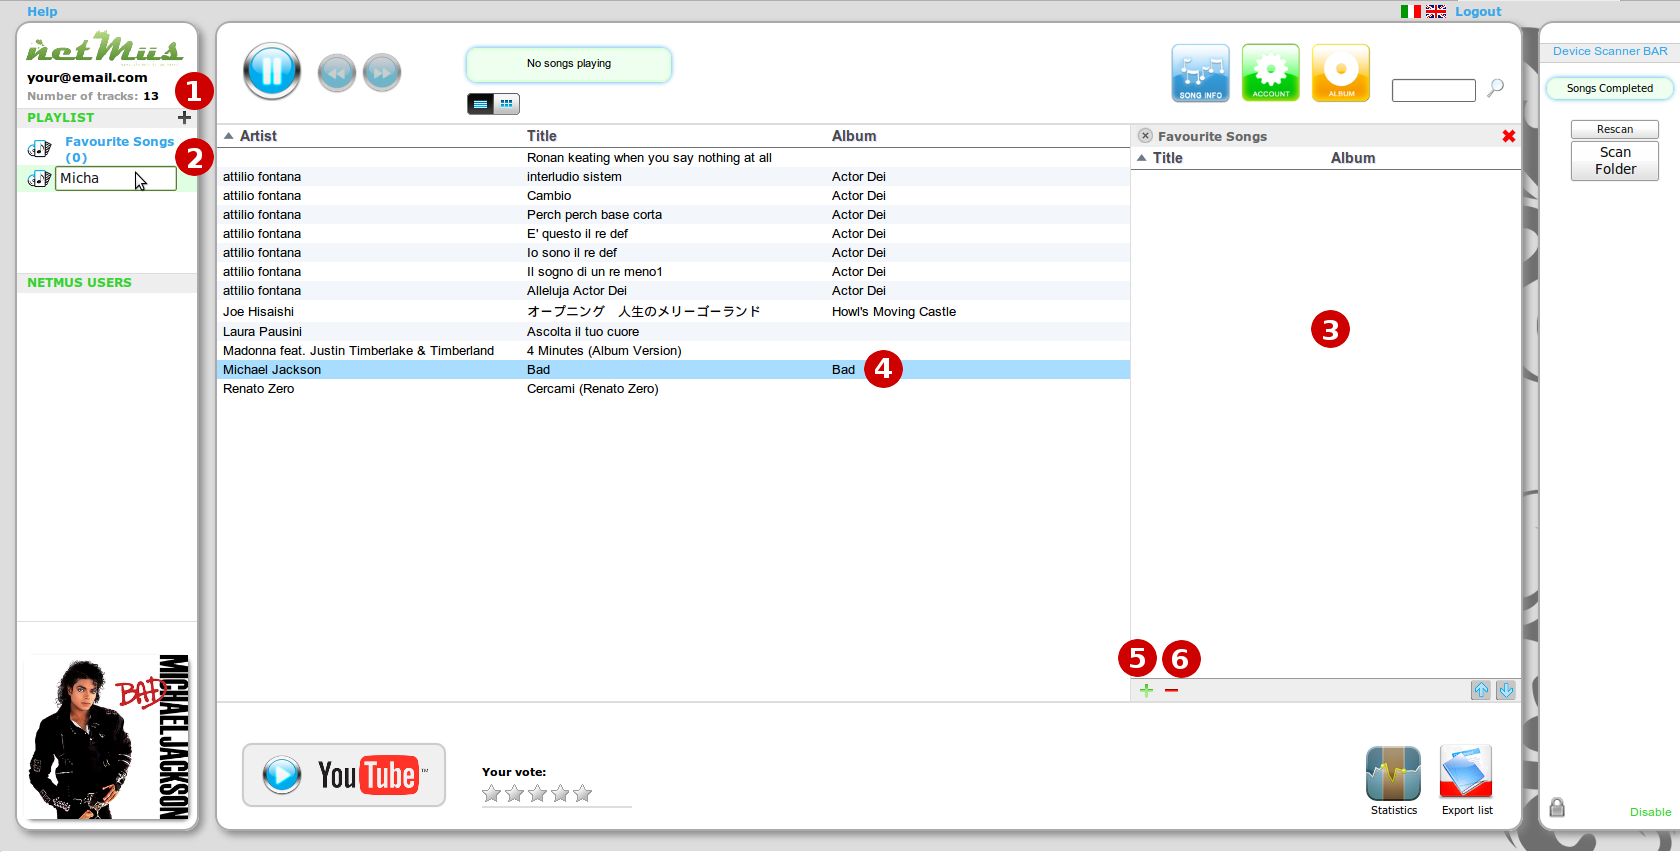
\includegraphics[width=15cm]{img/MU/new_playlist.png}\\
\caption{Pagina principale di NetMus con evidenziato men\`u di selezione
playlist}
\end{figure}
 
Ora non resta che inserire i brani all'interno della propria playlist
per ottenere la sequenza di canzoni desiderata. Per fare ci\`o basta cliccare sul
nome della playlist, si aprir\`a una finestrella (vuota per il momento) in cui
saranno presenti tutti i suoi brani. Per inserire un brano basta
selezionarlo e successivamente cliccare nella finestra della playlist il
simbolo ``+" verde.\\
La rimozione di un brano avviene in modo analogo; basta selezionare
nell'elenco dei brani della playlist il brano da rimuovere e successivamente
cliccare il simbolo ``-'' rosso.\\
Da notare che all'interno della finestrella con l'elenco dei brani della
playlist, una volta selezionato un brano dal catalogo multimediale o dalla
playlist le azioni di aggiunta di un brano sono scritte in verde, le azioni di
rimozione di un brano in rosso.\\
\begin{figure}[htbp]
  \centering
  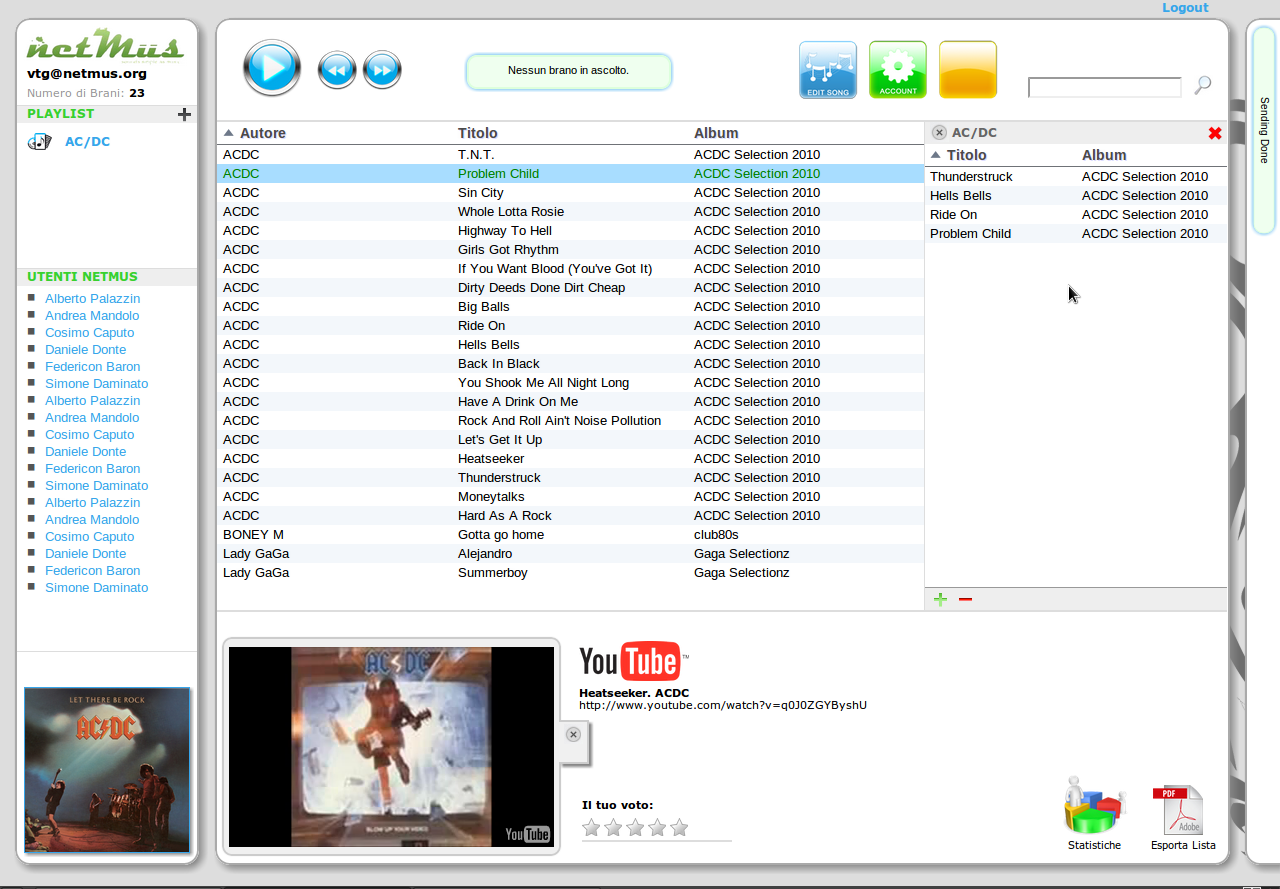
\includegraphics[width=15cm]{img/MU/playlist_song.png}\\
\caption{Dettaglio di una playlist}
\end{figure}

Infine per eliminare una playlist basta selezionarla e cliccare la ``X'' rossa che
si trova nella finestrella in alto a destra.

\subparagraph{Visualizzare le informazioni riguardanti un brano}

Per visualizzare ulteriori informazioni riguardanti un brano basta fare un
doppio click sopra lo stesso. Si aprir\`a una finestrella con l'elenco delle
informazioni riguardanti il brano.\\
\begin{figure}[htbp]
  \centering
  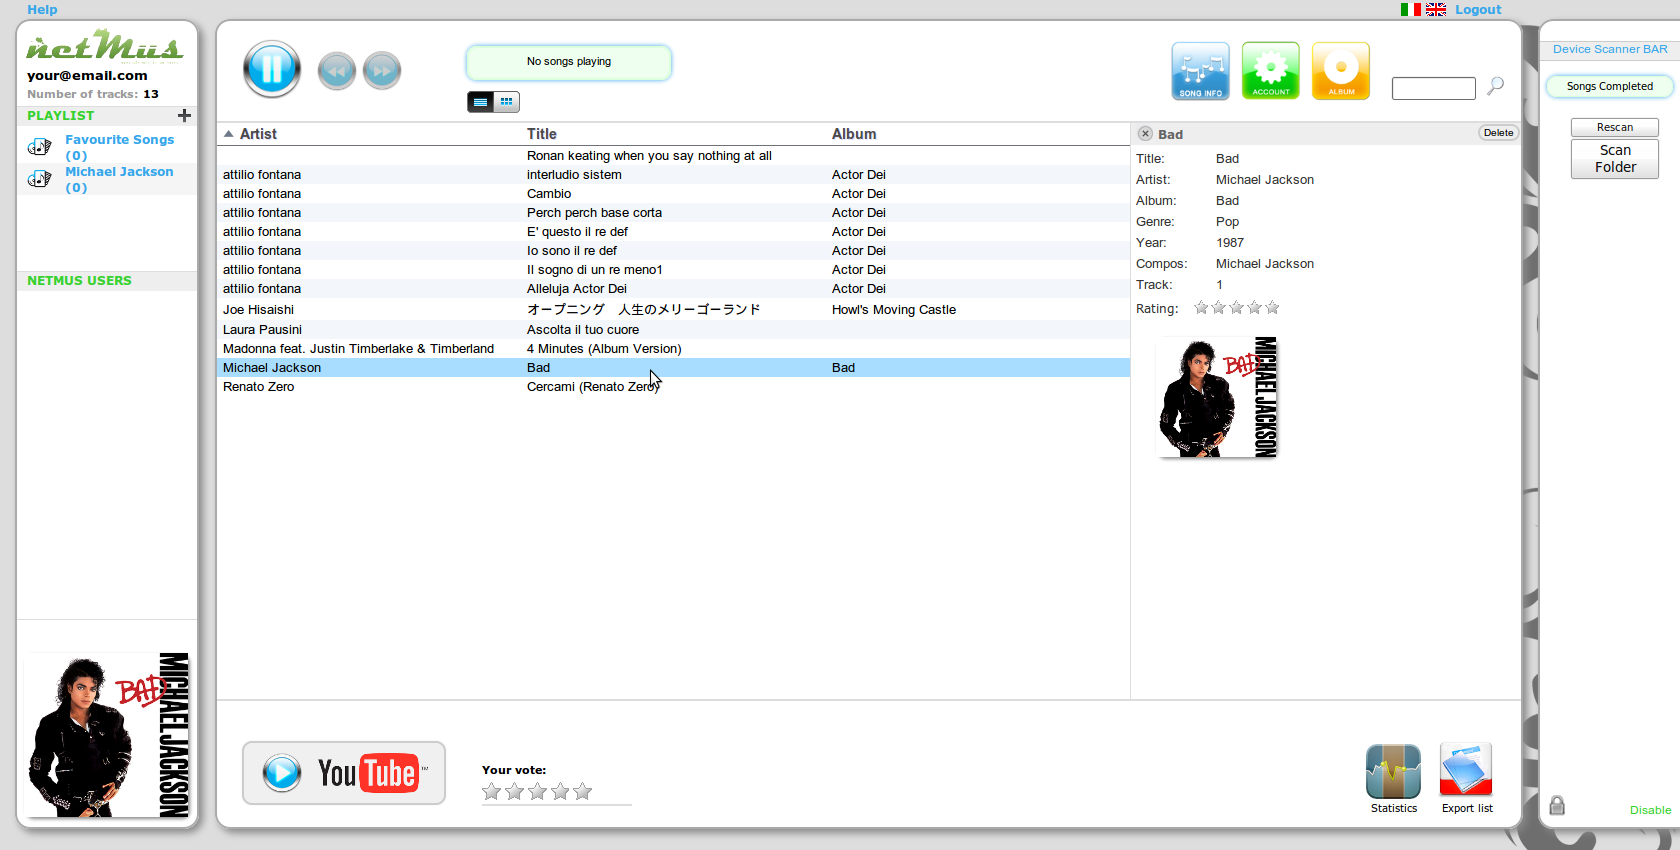
\includegraphics[width=15cm]{img/MU/info_song.png}\\
\caption{Dettagli di un brano del catalogo}
\end{figure}

Tra queste informazioni elenchiamo titolo, autore, album, genere, anno,
compositore, traccia, valutazione e copertina.\\
Per quanto riguarda la valutazione verr\`a spiegata pi\`u a fondo in seguito.\\
Le copertine invece vengono recuperate durante la memorizzazione del brano sul
catalogo.

\subparagraph{Eliminare un brano dal catalogo}

Per eliminare un brano dal proprio catalogo multimediale basta cliccarci sopra
due volte e fare apparire la finestrella con le informazioni dettagliate. A
questo punto cliccare la ``X'' rossa come per le playlist, e il brano verr\`a
immediatamente eliminato dall'elenco.

\subparagraph{Ricercare un brano sul catalogo}

Per la ricerca di un brano all'interno del catalogo \`e stata implementata una
\underline{form} apposita. La form, visualizzata nella pagina in alto a destra,
ci permette di ricercare titolo, album o artista di qualunque brano del catalogo.\\
La ricerca \`e immediata durante la digitazione, e i risultati vengono mostrati
direttamente sull'interfaccia principale del catalogo multimediale.

\subparagraph{Modificare le informazioni riguardanti un brano}

\emph{(Funzionalità che verrà integrata in una versione successiva.)}

\subparagraph{Modificare le informazioni del profilo (anche cambio password)}

Nel sistema \co{NetMus} \`e possibile compilare ulteriori campi riguardanti il
proprio profilo utente.\\
Tale operazione \`e possibile cliccando sul tasto verde ``Account''. Si aprir\`a
un pop-up con l'elenco dei campi che \`e possibile compilare. Le informazioni
dovranno essere inserite in tali form.
\begin{figure}[htbp]
  \centering
  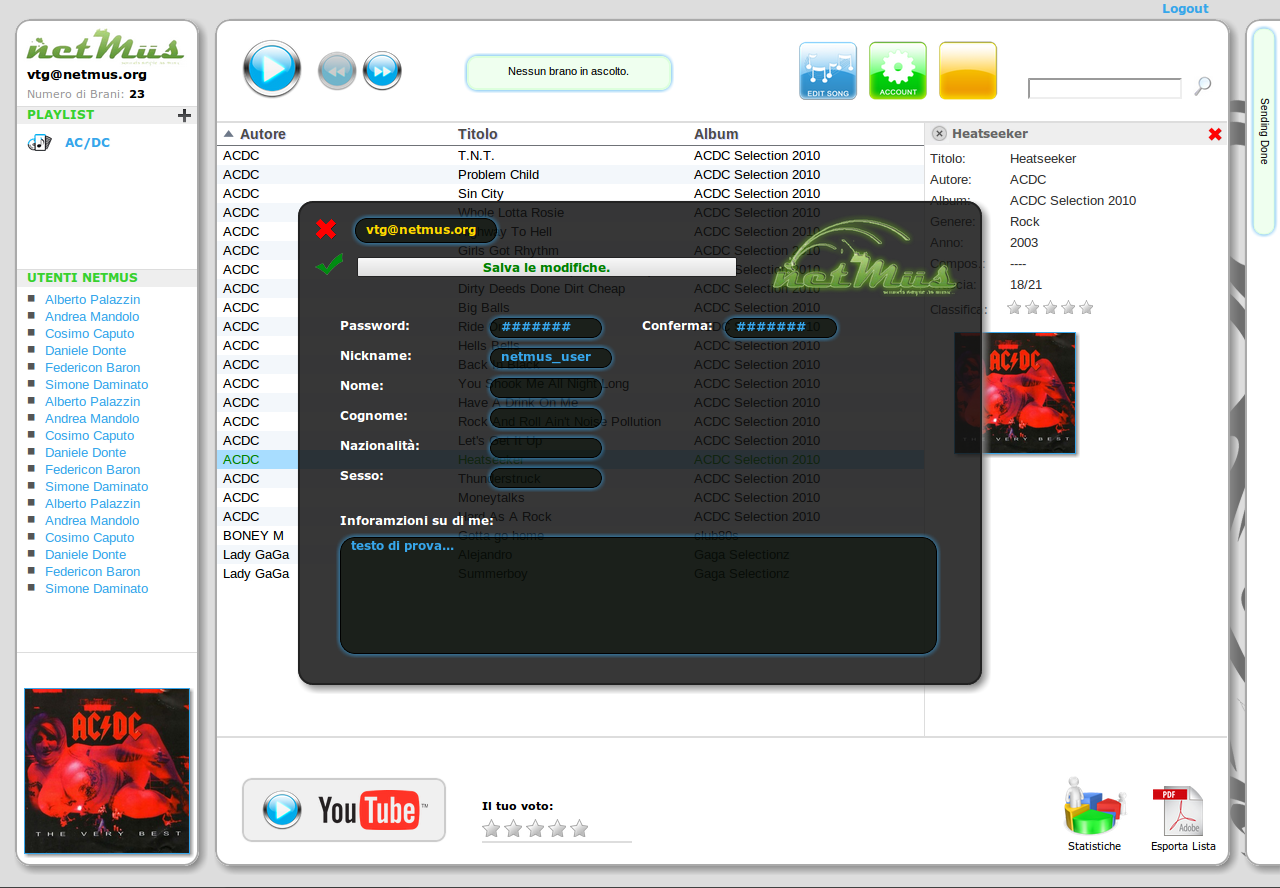
\includegraphics[width=15cm]{img/MU/profile_view.png}
\caption{Interfaccia per la modifica delle informazioni del profilo}
\end{figure}

Le informazioni che \`e possibile aggiungere sono nickname, nome, cognome,
nazionalit\`a, sesso e una breve descrizione di s\`e. Da questa interfaccia \`e
anche possibile cambiare la propria password.\\
Una volta inserite le nuove informazioni, cliccare su salva modifiche per
salvare quanto editato, o cliccare sulla ``X'' rossa per annullare.

\subparagraph{Dare un voto ad un brano}

Il sistema \co{NetMus} offre anche la possibilit\`a di valutare un brano su una
scala da 0 a 5 stelline.\\
Da notare che il voto espresso per il brano, verr\`a poi visualizzato nelle
informazioni del brano ma sottoforma di media di tutti i voti ricevuti dai
possessori all'interno del sistema \co{NetMus} di quella stessa canzone.\\
Per valutare un brano basta selezionarlo dal catalogo con un click, e
successivamente cliccare sul numero di stelline desiderato in basso. Il voto
verr\`a automaticamente registrato tra le informazioni del brano in questione.

\subparagraph{Esportare il proprio catalogo multimediale in PDF}

Questa funzione originale \`e stata inserita per permettere l'esportazione del
catalogo multimediale in un documento PDF, pi\`u adeguato alla stampa.\\
Per procedere con l'esportazione in PDF \`e necessario cliccare sul tasto in
basso a destra ``Esporta Lista''. A pressione avvenuta, il sistema
auto-generer\`a un PDF con l'elenco dei brani del catalogo, e aprir\`a una
finestra per far selezionare all'utente la directory in cui salvare il file PDF
creato.

\subparagraph{Visualizzare le statistiche del sistema e del proprio account}

Per visualizzare le statistiche del proprio sistema basta cliccare sul tasto
``Statistiche'' in basso a destra. Verranno dunque visualizzate su un pop-up le
statistiche riguardanti il sistema netmus(canzone pi\`u gettonata, numero di
utenti, ecc..) e le statistiche riguardanti il proprio account (canzone pi\`u
ascoltata, genere preferito, autore preferito, numero di amici ecc..).




\section{Errori probabili e cause possibili}

\subparagraph{Il dispositivo USB non viene analizzato}
\begin{itemize}
  \item controllare che la DEVICE SCANNER BAR non sia disabilitata. La DEVICE
  SCANNER BAR \`e disabilitata quando nell'angolo in basso vi \`e la scritta
  verde ``Enable''.
\end{itemize}

\subparagraph{Alcuni brani analizzati non sono stati caricati nel catalogo}
\begin{itemize}
  \item controllare che non fossero gi\`a stati analizzati e inseriti nel
  catalogo durante un' analisi precedente. Per essere sicuri, controllare il log
  presente all'interno del dispositivo in cui \co{NetMus} ha fatto la scansione.
  \item i brani non hanno i tag necessari completi. Se un brano non ha i
  tag artista titolo e album completi il brano non viene catalogato perch\`e non
  c'\`e modo di riconoscere quale brano sia.
  \item i brani contengono tag con codifica diversa dalla ISO-8859-1. Con i tag
  artista, titolo e album con caratteri diversi dalla codifica ISO-8859-1 i file
  vengono ignorati poich\`e \`e impossibile catalogarli dato che altre codifiche
  non vengono riconosciute e decifrate. Canzoni con i tag principali scritti ad
  esempio in Giapponese vengono ingnorate.
\end{itemize}

\subparagraph{La canzone riprodotta dal player di YouTube non \`e quella
corretta}
\begin{itemize}
  \item purtroppo la ricerca su YouTube non va sempre a buon fine. E possibile
  cliccare sul tasto ``Wrong Song'' per passare al video successivo dato dai
  risultati della ricerca su YouTube di tale canzone. Con tale funzionalit\`a la
  probabilit\`a di riprodurre il brano desiderato \`e maggiore.
  \item i tag delle canzone desiderata sono sbagliati e quindi la
  ricerca di tale canzone produce risultati errati. Modificare le informazioni
  della suddetta canzone per risolvere il problema.
\end{itemize}


\subparagraph{Password dimenticata}


\appendix % inizio appendice
\chapter{Messaggi di errore e loro significato}
\thispagestyle{fancy}

\chapter{Glossario}
\thispagestyle{fancy}

\section*{Browser web:} programma che consente all'utente di navigare in
Internet. 'Netscape' e 'Internet Explorer' sono dei browser. 
\section*{Cloud computing:} un insieme di tecnologie informatiche che
permettono l'utilizzo di risorse o software distribuite in remoto.
\section*{Directory:} cartella (del computer).
\section*{Dispositivi di archiviazione di massa:} hard disk esterni, penne
usb, lettori mp3, eccetera.
\section*{Form:} parte di un'interfaccia grafica, in genere uno o pi\`u campi
dove vanno inseriti dei dati. 
\section*{Nickname:} nome utente.
\section*{Player:} riproduttore multimediale.
\section*{Playlist:} \`e una lista di canzoni, utilizzata su
personal computer e media player portatili per la gestione pi\`u rapida dei
brani in esecuzione e la loro sequenza.
\section*{Social network:} comunit\`a on-line di persone che condividono
interessi e/o attivit\`a.
\section*{Streaming:} un flusso di dati audio/video trasmessi da una sorgente
a una o pi\`u destinazioni tramite una rete telematica. Questi dati vengono
riprodotti man mano che arrivano a destinazione.

\end{document}
